\begin{questions}
    \question{
        Explain, geometrically, the recursive formula for $nth$
        hexagonal number.
    }
    \begin{solution}
        To get $nth$ hexagonal number we add 4 sides each of size 
        $4n$. But since there are 3 common vertices for the added
        4 sides, we subtract 3.
        Hence the recursive definition of the hexagonal numbers 
        are given by:
        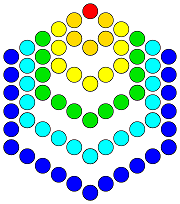
\includegraphics[width=0.25\textwidth]{images/hex.png}
        $$h_1=1, \quad h_n=h_{n-1}+4n-3$$
    \end{solution}
    \question{
        .
    }
    \begin{solution}
        $$h_n=n(2n-1),\quad n\ge 1$$
        We see that $h(1)=1$, which is true. So let the statement
        $$H_k: h_k=k(2k-1)$$ be true for some integer $k>1$. Then,
        \begin{align*}
            h_{k+1}&=h_k+4(k+1)-3\\
            &=2k^2-k+4k+4-3\\
            &=2k^2+3k+1\\
            &=(2k+1)(k+1)\\
            &=\left(k+1\right)\left(2(k+1)-1\right)
        \end{align*}
        Then since $H_k\implies H_{k+1}$, the statement is true for
        all $k\in\mathbf{N}$
    \end{solution}
\end{questions}